\chapter{Tests, sécurité, DevOps et déploiement Azure}
\label{chap:tests-securite}

\section*{Introduction}

Après la réalisation de la plateforme, sa valeur dépend autant de la fiabilité de la chaîne complète que de la cohérence du moteur de rapprochement. Ce chapitre présente les contrôles effectivement disponibles dans JobTest, les vérifications effectuées lors du déploiement et les protections visibles dans le code et la configuration. Il distingue les tests automatisés, les vérifications manuelles et les observations ponctuelles faites sur la machine de démonstration. L'objectif n'est pas de certifier une disponibilité de production, mais de documenter de manière traçable le périmètre validé, les choix d'exploitation et les limites restantes.

\section{Stratégie de validation}

La validation combine une suite \texttt{pytest}, des contrôles d'API et une vérification de bout en bout sur l'environnement conteneurisé. Les essais de benchmark du chapitre 4 restent séparés : ils étudient un corpus synthétique et ne constituent pas une suite de tests fonctionnels. Le tableau \ref{tab:chap6-validation-strategy} synthétise le statut des éléments examinés.

\begin{table}[H]
\centering
\small
\caption{Niveaux de validation retenus pour JobTest}
\label{tab:chap6-validation-strategy}
\begin{tabularx}{\textwidth}{|p{.12\textwidth}|p{.18\textwidth}|X|p{.14\textwidth}|}
\hline
\textbf{Niveau} & \textbf{Objectif} & \textbf{Outil ou méthode} & \textbf{Statut}\\
\hline
Unitaires & Vérifier extraction, fusion, décision, PDF et règles de cohérence. & \texttt{pytest} ; modèles de langue et Ollama simulés lorsque nécessaire. & Partiel : 106 réussites sur 113 items.\\
\hline
API et intégration & Vérifier routes, statuts HTTP, JWT, persistance et contrats. & Tests FastAPI et contrôles d'API documentés. & Partiel : 6 tests hérités à adapter.\\
\hline
Fonctionnel & Vérifier le parcours recruteur depuis l'inscription jusqu'au rapport. & Scénario manuel enregistré sur la VM Azure. & Réalisé sur un jeu synthétique.\\
\hline
Chaîne IA & Vérifier sous-scores, verdict, explication et statut de la couche 2. & Tests du moteur, réponses de l'API et contrôle du résultat persistant. & Réalisé ; benchmark distinct au chapitre 4.\\
\hline
Déploiement & Vérifier les conteneurs, le proxy, les health checks et les ports. & \texttt{docker compose}, \texttt{nginx -t}, requêtes HTTP et journaux. & Réalisé ponctuellement.\\
\hline
\end{tabularx}
\end{table}

Le dernier lancement documenté de \texttt{pytest -q} a produit 106 tests réussis, 6 échecs et 1 test ignoré (113 items, environ 45 secondes). Les six échecs sont concentrés dans \texttt{test\_api\_extended.py} : des fixtures de routes historiques ne satisfont plus le contrôle d'appartenance introduit pour les offres et résultats. Ils retournent donc \texttt{404} au lieu du résultat attendu par ces tests anciens. Ce constat ne permet pas de déclarer la suite entièrement verte ; sa mise à jour constitue une action de maintenance.

\section{Environnement et données de test}

Le développement a été conduit localement sous Windows avec Python, Node.js et SQLite, puis vérifié dans une topologie Docker Compose utilisant PostgreSQL. La validation intégrée a ensuite été observée sur une machine virtuelle Azure. Les parcours fonctionnels ont utilisé un compte recruteur de démonstration, une offre et un CV synthétiques. Aucun résultat présenté dans ce chapitre ne requiert l'affichage d'un mot de passe, d'un jeton, d'une clé SSH, d'une chaîne de connexion ou du contenu du fichier \texttt{.env}. Les éléments visibles dans les traces de déploiement sont des données de vérification et non un jeu de CV réels.

\section{Tests fonctionnels}

La matrice suivante reprend seulement les scénarios dont l'exécution ou le résultat est attesté par les tests du dépôt ou le rapport de déploiement. Les cas non exécutés ne sont pas convertis artificiellement en succès.

Le tableau~\ref{tab:chap6-functional-matrix} en dresse la liste.

{\scriptsize
\begin{longtable}{|p{.06\textwidth}|p{.18\textwidth}|p{.19\textwidth}|p{.23\textwidth}|p{.18\textwidth}|p{.08\textwidth}|}
\caption{Matrice des contrôles fonctionnels attestés}\label{tab:chap6-functional-matrix}\\
\hline
\textbf{ID} & \textbf{Fonction} & \textbf{Précondition} & \textbf{Résultat attendu} & \textbf{Résultat obtenu} & \textbf{Statut}\\
\hline
\endfirsthead
\hline
\textbf{ID} & \textbf{Fonction} & \textbf{Précondition} & \textbf{Résultat attendu} & \textbf{Résultat obtenu} & \textbf{Statut}\\
\hline
\endhead
F01 & Inscription et connexion & Compte de vérification. & Création puis obtention d'un jeton sans l'exposer. & Compte créé et JWT utilisé pendant la vérification Azure. & OK\\
\hline
F02 & Refus d'identifiants invalides & Identifiants incorrects. & Réponse d'authentification refusée. & Couvert par les tests \texttt{test\_auth}. & OK\\
\hline
F03 & Consultation du profil & Jeton Bearer valide. & Retour du recruteur connecté. & Route protégée couverte par les tests d'authentification. & OK\\
\hline
F04 & Création d'offre & Recruteur authentifié. & Offre enregistrée et rattachée au recruteur. & Offre de contrôle créée (identifiant 1 dans l'environnement observé). & OK\\
\hline
F05 & Évaluation d'un CV & Offre et CV de démonstration. & Sous-scores, explication et recommandation générés. & Résultat \texttt{MatchResult} 1 créé, verdict \texttt{CONSIDER}. & OK\\
\hline
F06 & Persistance & Évaluation réussie. & Résultat récupérable avec relations cohérentes. & Un résultat et une analyse LLM valide comptabilisés dans PostgreSQL. & OK\\
\hline
F07 & Analyse approfondie & Résultat persistant, Ollama disponible. & Enveloppe d'analyse sans modification du score. & \texttt{status=ok} observé et analyse enregistrée. & OK\\
\hline
F08 & Rapport PDF & Résultat calculé. & Flux PDF ouvrable avec informations d'évaluation. & PDF 1.4, deux pages et 112\,039 octets dans ce cas. & OK\\
\hline
F09 & Routes API historiques & Fixtures anciennes de test. & Réponse des routes historiques. & Six attentes sont incompatibles avec le contrôle de propriété. & À adapter\\
\hline
\end{longtable}
}

\section{Validation du moteur intelligent}

Le contrôle fonctionnel du moteur concerne ici sa mise en œuvre, non la qualité prédictive discutée au chapitre 4. Une évaluation retournée par l'API contient les trois sous-scores utilisés dans la fusion, les paramètres de pondération, l'explication structurée et la recommandation algorithmique. Les tests couvrent la fusion hybride, les frontières de décision, la cohérence entre moteur et module d'explication ainsi que les états \texttt{disabled}, \texttt{unavailable}, \texttt{error}, \texttt{ok} et \texttt{inconsistent} de la couche 2.

La couche générative reçoit le résultat déterministe mais ne calcule ni le score officiel ni le verdict \texttt{HIRE}, \texttt{CONSIDER} ou \texttt{REJECT}. Les tests de raisonnement emploient un Ollama simulé ; la disponibilité réelle de la couche 2 a, elle, été vérifiée une fois sur Azure. Les cas de CV vide, d'offre inexistante et de ressources appartenant à un autre recruteur sont contrôlés par les routes concernées. Les résultats de cas de seuil exact 55 ou 75 ne sont pas présentés séparément ici, faute de trace de démonstration dédiée.

\section{Tests de l'API et de la persistance}

Les schémas Pydantic valident les corps de requête et FastAPI retourne notamment des erreurs \texttt{401}, \texttt{404}, \texttt{422} ou \texttt{429} selon le contrat concerné. Chaque route de données passe par l'authentification Bearer. La fonction \texttt{\_assert\_owned} vérifie que l'offre et le candidat visés appartiennent au recruteur connecté ; une ressource d'un autre périmètre est traitée comme absente. Les requêtes courantes sont exprimées par SQLAlchemy plutôt que par concaténation de SQL ; cette pratique réduit l'exposition à des chaînes SQL construites manuellement, sans constituer à elle seule une garantie universelle.

La vérification Azure a confirmé l'écriture d'un \texttt{MatchResult} et d'une analyse LLM valide, puis leur comptage dans PostgreSQL. Les relations candidat, offre et résultat ont donc été parcourues dans un scénario réel de démonstration. Swagger était accessible derrière Nginx à \texttt{/api/v1/docs}; aucune capture n'est ajoutée afin d'éviter de répéter les écrans du chapitre 5.

\section{Validation du rapport PDF}

La génération est testée dans le dépôt par des contrôles de structure binaire et a également été validée dans le parcours déployé. Pour un résultat précis, la réponse HTTP a été reçue sous forme de PDF 1.4, le fichier s'est ouvert sur deux pages et sa taille était de 112\,039 octets. Ces valeurs caractérisent un exemple de démonstration : le nombre de pages et le poids peuvent évoluer avec les données du candidat et de l'offre. L'export utilise les informations déjà calculées ; il ne lance pas un nouveau rapprochement.

\section{Tests de santé et stabilité des services}

Les cinq conteneurs ont été observés à l'état \emph{healthy}, avec une politique \texttt{unless-stopped} et sans redémarrage inattendu lors du contrôle. La configuration Nginx a passé \texttt{nginx -t}; l'accueil et Swagger ont retourné HTTP 200 via le proxy. L'endpoint FastAPI de santé et son contrôle détaillé ont retourné \texttt{ok}; la couche 1 était disponible, Ollama répondait et le modèle \texttt{qwen2.5:1.5b} était installé. Les journaux examinés ne montraient ni OOM, ni erreur fatale, ni boucle de redémarrage. Il s'agit d'une observation à un instant donné et non d'un engagement de disponibilité permanente.

\section{Résultats de validation de bout en bout}

Le scénario intégré attesté suit les étapes suivantes : utilisation d'un compte recruteur, authentification, création d'une offre, évaluation d'un CV synthétique, enregistrement du résultat, lecture de l'explication, analyse approfondie puis génération du PDF servi par Nginx. Cette chaîne a produit les trois composantes de score, une recommandation \texttt{CONSIDER}, un \texttt{MatchResult} persistant, une analyse LLM \texttt{ok} et le rapport PDF décrit précédemment.

La mesure de l'analyse approfondie est de 54\,290,6 ms sur cette VM CPU. Elle doit être interprétée comme une mesure ponctuelle sur une infrastructure de démonstration et non comme un objectif de temps de réponse. La couche 1 demeurait opérationnelle pendant que la couche qualitative est, par conception, additive et consultative.

\section{Sécurité applicative}

Les mots de passe sont traités par \texttt{passlib} avec le schéma \texttt{bcrypt} visible dans le code. Les jetons JWT sont signés en HS256, portent une expiration et sont vérifiés à chaque dépendance \texttt{get\_current\_user}. La clé provient de l'environnement ; en son absence, l'application fabrique une valeur aléatoire au démarrage, ce qui invalide les sessions au redémarrage et produit un avertissement. En déploiement, une valeur durable est donc fournie hors dépôt.

La séparation par \texttt{recruiter\_id}, les contrôles de propriété et les schémas Pydantic constituent les protections principales des opérations métier. Les fichiers sont acceptés selon l'extension PDF/DOCX et passent par un fichier temporaire ; Nginx limite le corps des requêtes à 15 Mo. Cette dernière limite ne remplace pas une validation de signature de fichier : celle-ci n'est pas implémentée. Un limiteur en mémoire applique par défaut 60 requêtes par minute et par adresse ; il ne remplace ni une politique de verrouillage de compte ni une protection distribuée.

Les secrets réels sont exclus du dépôt et des contextes Docker. La configuration de la VM place \texttt{/opt/jobtest/.env} avec le mode 0600 observé. Les erreurs de la couche LLM sont ramenées à une enveloppe d'état contrôlée : la chaîne statistique reste utilisable si Ollama est indisponible. Ces mécanismes sont des mesures concrètes, mais ne justifient aucune revendication de conformité ou de sécurité totale.

\section{Sécurité réseau et infrastructure}

Un groupe de sécurité réseau Azure (NSG) filtre le trafic entrant et sortant au niveau des ressources virtuelles ; ses règles peuvent notamment spécifier le protocole, le port, l'action et la priorité \cite{azure_nsg}. Dans le déploiement observé, une règle effective autorise HTTP TCP 80 et SSH TCP 22 est ouvert pour l'administration. Les détails administratifs de la règle (nom, priorité et association exacte) n'ont pas été récupérés depuis le portail Azure et ne sont donc pas reconstitués.

Nginx est le seul conteneur publiant un port hôte. Il relaie \texttt{/api/v1/} vers FastAPI et les autres chemins vers Next.js. Compose attache les services au réseau \texttt{jobtest} de type bridge ; ils sont joignables par leurs noms de service, tandis qu'un port hôte n'est nécessaire que pour l'accès extérieur \cite{docker_compose_networking}. Ainsi, 3000, 8000, 5432 et 11434 ne sont pas publiquement exposés. UFW a été observé inactif sur la VM : l'isolation actuelle repose donc sur le NSG, l'absence de mappings de ports et le proxy, plutôt que sur une seconde couche active de filtrage local.

\begin{figure}[H]
\centering
\begin{tikzpicture}[scale=.83, transform shape, node distance=7mm and 8mm]
\node[archbox, fill=gray!12] (client) {Poste du\\recruteur};
\node[archbox, right=of client, fill=cyan!8] (nsg) {Internet\\Azure NSG\\TCP 80 / SSH 22};
\node[archbox, right=of nsg, fill=green!8] (nginx) {VM Ubuntu\\Nginx :80};
\node[archbox, below left=13mm and 10mm of nginx] (web) {Next.js\\:3000};
\node[archbox, below=13mm of nginx] (api) {FastAPI\\:8000};
\node[datastore, below right=13mm and 10mm of api] (db) {PostgreSQL\\:5432\\postgres\_data};
\node[archbox, right=of api] (ollama) {Ollama\\:11434\\ollama\_data};
\node[draw=isiBlue, rounded corners=4pt, fit=(nginx)(web)(api)(db)(ollama), inner sep=8mm, label={[font=\footnotesize]above:Réseau Docker \texttt{jobtest}}] (docker) {};
\node[draw=black!60, rounded corners=5pt, fit=(nginx)(docker), inner sep=11mm, label={[font=\footnotesize]above:Machine virtuelle Ubuntu}] (vm) {};
\node[draw=isiBlue, dashed, rounded corners=6pt, fit=(nsg)(vm), inner sep=12mm, label={[font=\footnotesize]above:Microsoft Azure --- East US}] (azure) {};
\draw[umlrel,-{Stealth[length=2mm]}] (client) -- node[above,font=\scriptsize]{HTTP} (nsg);
\draw[umlrel,-{Stealth[length=2mm]}] (nsg) -- (nginx);
\draw[umlrel,-{Stealth[length=2mm]}] (nginx) -- node[left,font=\scriptsize]{routes Web} (web);
\draw[umlrel,-{Stealth[length=2mm]}] (nginx) -- node[right,font=\scriptsize]{\texttt{/api/v1}} (api);
\draw[umlrel,-{Stealth[length=2mm]}] (api) -- (db);
\draw[umlrel,-{Stealth[length=2mm]}] (api) -- (ollama);
\end{tikzpicture}
\caption{Architecture concrète de déploiement : accès public, VM et réseau Docker interne}
\label{fig:chap6-deployment}
\end{figure}

\section{Analyse honnête des limites de sécurité}

Le démonstrateur utilise HTTP, sans domaine ni certificat TLS. Le jeton Bearer est conservé côté frontend dans \texttt{localStorage}; une injection de script réussie pourrait donc le lire. OWASP recommande de ne pas placer de données sensibles dans ce stockage lorsque des attaques XSS sont à considérer \cite{owasp_html5_storage}. Un passage vers des cookies \texttt{HttpOnly}, \texttt{Secure} et \texttt{SameSite} est une amélioration souhaitable, associée à une protection XSS approfondie.

Le port SSH exposé doit être limité à une adresse d'administration connue ; \texttt{fail2ban} peut compléter cette mesure selon le contexte. Aucune rotation automatisée des secrets, aucun WAF, aucune supervision centralisée ni sauvegarde PostgreSQL planifiée ne sont attestés. L'infrastructure n'a qu'une VM, une base et un point d'entrée : elle ne fournit ni haute disponibilité ni reprise automatisée. Les téléversements restent perfectibles (contrôle de type fondé surtout sur l'extension, pas de validation par signature), et les textes envoyés à la couche LLM doivent être considérés comme non fiables. Une politique de conservation, d'anonymisation et de suppression contrôlée des CV est également nécessaire avant un emploi sur des candidatures réelles.

\section{Traitement des données à caractère personnel}

Un CV n'est pas un document technique ordinaire : il identifie une personne et décrit son parcours. Toute plateforme qui l'ingère traite donc des données à caractère personnel, et il serait malhonnête de discuter la sécurité de JobTest sans nommer cette dimension. Les catégories manipulées par la plateforme sont l'identité déclarée du candidat, son adresse électronique et son téléphone lorsqu'ils figurent dans le dossier, le texte intégral du CV avec les employeurs, établissements et dates qu'il contient, puis les données produites par le système lui-même : score, verdict, compétences détectées ou absentes et analyse qualitative éventuelle. Cette dernière catégorie mérite attention, car une appréciation calculée sur une personne devient à son tour une donnée la concernant.

Le cadre applicable en Tunisie est la loi organique n\textsuperscript{o}~2004-63 du 27~juillet 2004 relative à la protection des données à caractère personnel \cite{loi2004_63}. Sans en reprendre le détail, son économie générale repose sur quelques principes : le traitement suppose en règle générale le consentement de la personne concernée, il doit poursuivre une finalité déterminée et légitime, les données collectées doivent rester en rapport avec cette finalité, et la personne conserve des droits d'accès, de rectification et de suppression sur ce qui la concerne. La loi institue également une autorité de contrôle, l'Instance nationale de protection des données à caractère personnel, chargée de recevoir les déclarations de traitement, de délivrer les autorisations prévues par le texte et d'instruire les réclamations \cite{inpdp}. Un usage réel de JobTest sur des candidatures authentiques relèverait de ce cadre et supposerait les démarches correspondantes auprès de cette instance ; le présent projet, conduit sur des CV synthétiques dans un contexte académique, ne les a pas engagées.

Plusieurs choix d'architecture décrits dans ce mémoire ont néanmoins un effet direct sur la protection des candidats, et il est utile de les relire sous cet angle plutôt que de les présenter comme de simples mesures techniques. Le cloisonnement par \texttt{recruiter\_id} fait qu'un dossier n'est lisible que dans l'espace du recruteur qui l'a créé : une offre ou un candidat appartenant à un autre compte est traité comme inexistant, ce qui limite la circulation interne des données. L'exécution locale du modèle de langage est le second point notable : la couche~2 s'adresse à un conteneur Ollama joint par le réseau interne, de sorte que le contenu d'un CV n'est jamais transmis à un fournisseur d'intelligence artificielle externe, contrairement à ce qu'impliquerait l'appel d'une API tierce. Enfin, la suppression d'un dossier candidat est une action exposée par l'interface, ce qui fournit un premier support à une demande d'effacement, même si sa portée reste bornée par la règle qui protège l'historique des évaluations.

Ces éléments sont des dispositions de conception, non une mise en conformité. Plusieurs exigences que la loi rend centrales ne sont pas couvertes par la version étudiée : aucun mécanisme de recueil ni de preuve du consentement n'existe, puisque le candidat n'interagit jamais avec la plateforme ; aucune durée de conservation n'est définie ni appliquée automatiquement aux CV et aux résultats ; aucune information n'est délivrée à la personne évaluée sur l'existence du traitement ou sur la logique du score qui la concerne ; et la démonstration circule en HTTP, sans chiffrement du transport. À cela s'ajoute que le texte d'un CV est conservé intégralement dans la base, alors qu'une partie de son contenu n'est pas nécessaire au calcul de correspondance.

Les travaux à mener avant tout usage sur des candidatures réelles se déduisent de cette liste : définir et appliquer une durée de conservation avec purge automatique, informer les candidats et organiser le recueil de leur consentement par le recruteur, réduire les données stockées à ce que le rapprochement exige réellement, ouvrir une voie d'exercice des droits d'accès et de suppression, chiffrer le transport, et effectuer les formalités requises auprès de l'autorité de contrôle. Ces points ne sont pas des perspectives lointaines mais des conditions d'entrée en service ; les mentionner explicitement vaut mieux que de laisser croire qu'un prototype validé techniquement serait, pour cette raison, utilisable sur des personnes.

\section{Conteneurisation}

Docker Compose décrit cinq services et les volumes nommés qui conservent les données hors du cycle de vie d'un conteneur. Les Dockerfiles de l'API et de Next.js construisent respectivement les images applicatives ; les images Nginx, PostgreSQL et Ollama sont référencées par Compose. Les dépendances conditionnent le démarrage de l'API à la santé de PostgreSQL, et celui de Nginx à la santé de l'API et du frontend. Les health checks contrôlent l'API, la page web, \texttt{pg\_isready}, \texttt{ollama list} et la réponse HTTP locale de Nginx.

Le tableau~\ref{tab:chap6-containers} précise le rôle, le port et la persistance de chacun d'eux.

\begin{table}[H]
\centering
\small
\caption{Services conteneurisés de JobTest}
\label{tab:chap6-containers}
\begin{tabularx}{\textwidth}{|p{.13\textwidth}|p{.20\textwidth}|X|p{.10\textwidth}|p{.16\textwidth}|}
\hline
\textbf{Conteneur} & \textbf{Image ou build} & \textbf{Rôle} & \textbf{Port} & \textbf{Persistance}\\
\hline
Nginx & \texttt{nginx:1.27-alpine} & Entrée HTTP et proxy inverse. & 80 public & Configuration montée en lecture seule.\\
\hline
Web & Build \texttt{web/Dockerfile} & Interface Next.js. & 3000 interne & Aucune donnée métier.\\
\hline
API & Build \texttt{Dockerfile.api} & API, moteur et génération PDF. & 8000 interne & \texttt{embedding\_cache}.\\
\hline
PostgreSQL & \texttt{postgres:16-alpine} & Base relationnelle. & 5432 interne & \texttt{postgres\_data}.\\
\hline
Ollama & \texttt{ollama/ollama:0.5.13} & Analyse qualitative locale. & 11434 interne & \texttt{ollama\_data}.\\
\hline
\end{tabularx}
\end{table}

\section{Déploiement sur Microsoft Azure}

Le déploiement a suivi un enchaînement simple : création du groupe de ressources, création de la VM Ubuntu, accès SSH, préparation de Docker, transfert de la version retenue, création locale du fichier \texttt{.env}, construction des images, téléchargement du modèle Ollama, démarrage Compose puis vérification des services et de Nginx. Le port HTTP a été ouvert de façon contrôlée pour la démonstration. La VM \texttt{vm-jobtest-pfe}, dans le groupe \texttt{rg-jobtest-pfe}, est localisée en East US. L'instance publique de démonstration est accessible à l'adresse \url{http://20.51.167.202/}. Cette adresse ne doit pas être considérée comme stable en cas de désallocation ou de redémarrage de la VM.

\begin{center}
\small\textbf{QR code d'accès à la démonstration publique de JobTest}\\[2mm]
\qrcode[height=2.8cm]{http://20.51.167.202/}\\[1mm]
\url{http://20.51.167.202/}
\end{center}

\begin{table}[H]
\centering
\small
\caption{Configuration observée de la machine virtuelle de démonstration}
\label{tab:chap6-azure-vm}
\begin{tabularx}{\textwidth}{|p{.30\textwidth}|X|}
\hline
\textbf{Paramètre} & \textbf{Valeur observée ou déclarée dans le rapport de déploiement}\\
\hline
Fournisseur et région & Microsoft Azure, East US.\\
\hline
Machine et système & \texttt{vm-jobtest-pfe}, Ubuntu Server 24.04 LTS.\\
\hline
Taille & Standard D2as\_v7 ; 2 vCPU et 8 Gio de mémoire.\\
\hline
Stockage et mémoire virtuelle & Disque Standard SSD ; swap persistante de 4 Gio.\\
\hline
Accès & HTTP TCP 80 public ; SSH TCP 22 pour l'administration.\\
\hline
Arrêt automatique & Configuré autour de 02 h, fuseau \emph{W. Europe Standard Time}.\\
\hline
\end{tabularx}
\end{table}

Les captures du portail Azure ci-dessous sont recadrées afin de ne pas afficher l'adresse e-mail de connexion ni l'identifiant d'abonnement. Elles constituent des constats visuels de l'environnement de démonstration et complètent les valeurs synthétisées dans le tableau \ref{tab:chap6-azure-vm}.

La figure~\ref{fig:chap6-azure-subscription} présente l'abonnement utilisé pour la démonstration.

\begin{figure}[H]
  \centering
  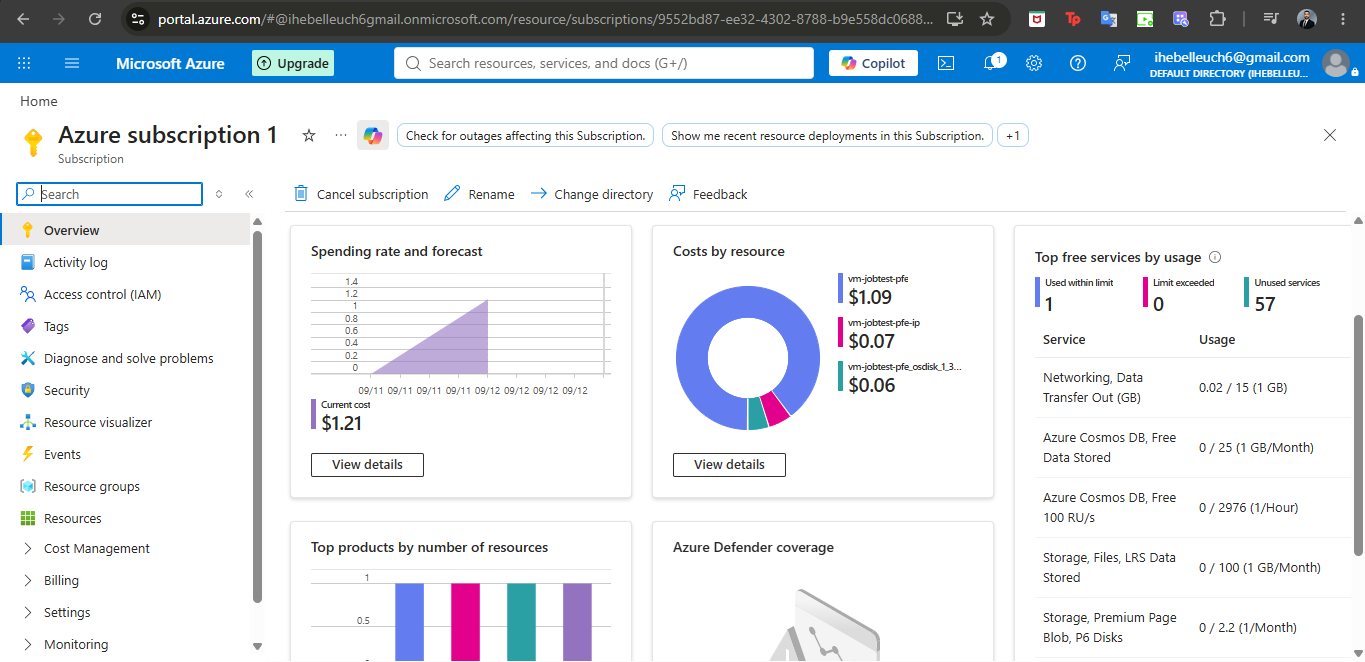
\includegraphics[width=.82\textwidth,trim=0 0 0 105bp,clip]{img/azure/azure_subscription.png}
  \caption{Vue de l'abonnement Azure, recadrée}
  \label{fig:chap6-azure-subscription}
\end{figure}

La figure~\ref{fig:chap6-azure-overview} donne l'aperçu de consommation associé.

\begin{figure}[H]
  \centering
  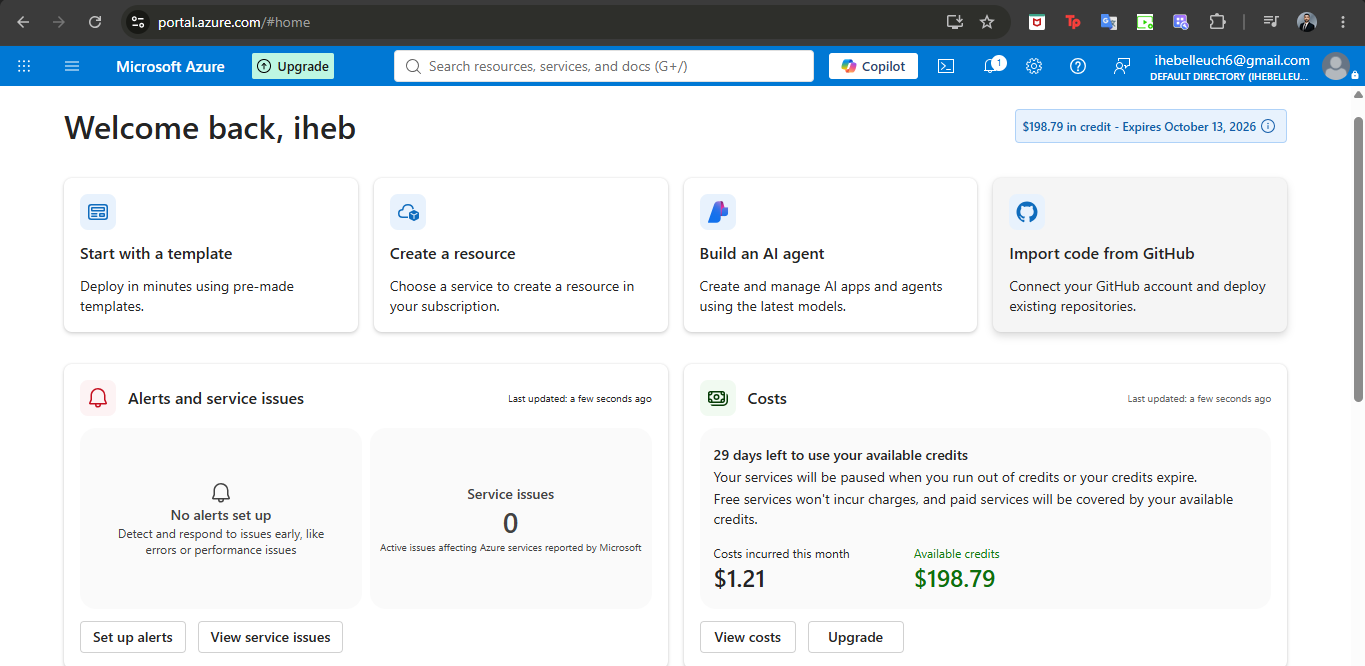
\includegraphics[width=.82\textwidth,trim=0 0 0 170bp,clip]{img/azure/azure_overview.png}
  \caption{Aperçu de consommation Azure, recadré}
  \label{fig:chap6-azure-overview}
\end{figure}

Les ressources créées pour le projet sont visibles sur la figure~\ref{fig:chap6-azure-resources}.

\begin{figure}[H]
  \centering
  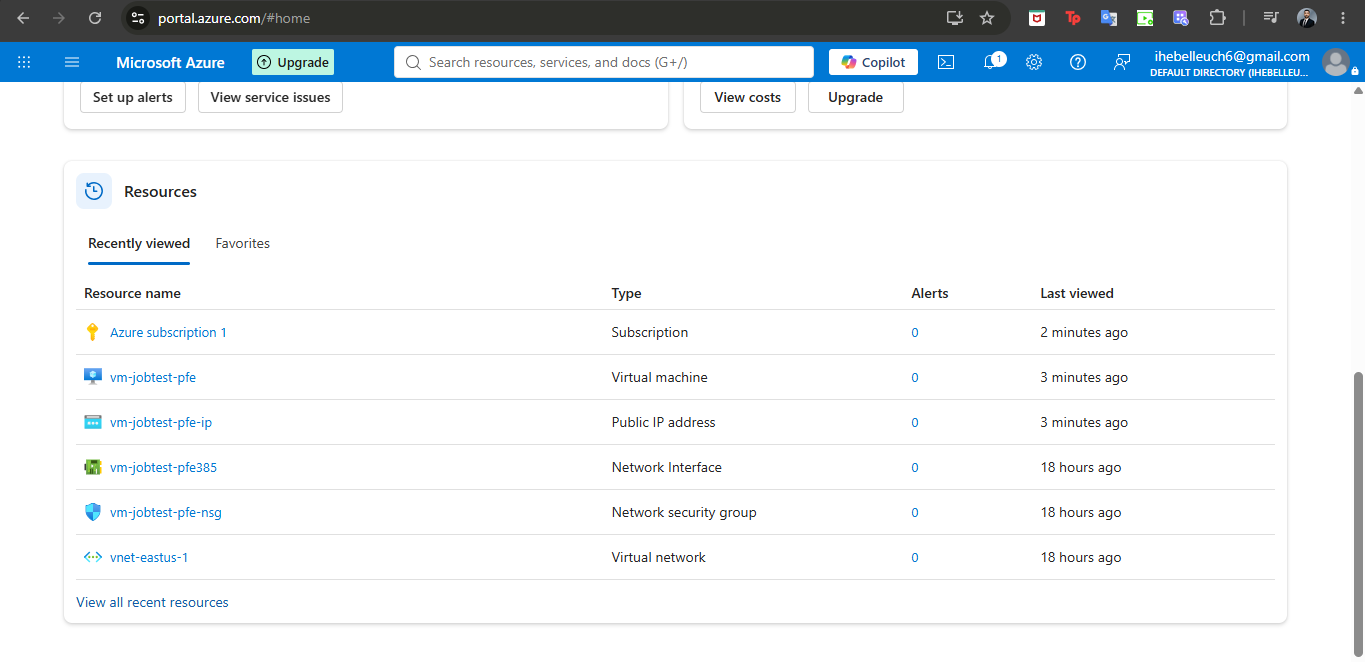
\includegraphics[width=.82\textwidth,trim=0 0 0 105bp,clip]{img/azure/azure_ressources.png}
  \caption{Ressources Azure associées à la démonstration}
  \label{fig:chap6-azure-resources}
\end{figure}

La figure~\ref{fig:chap6-azure-vm-properties} reprend les propriétés de la machine virtuelle.

\begin{figure}[H]
  \centering
  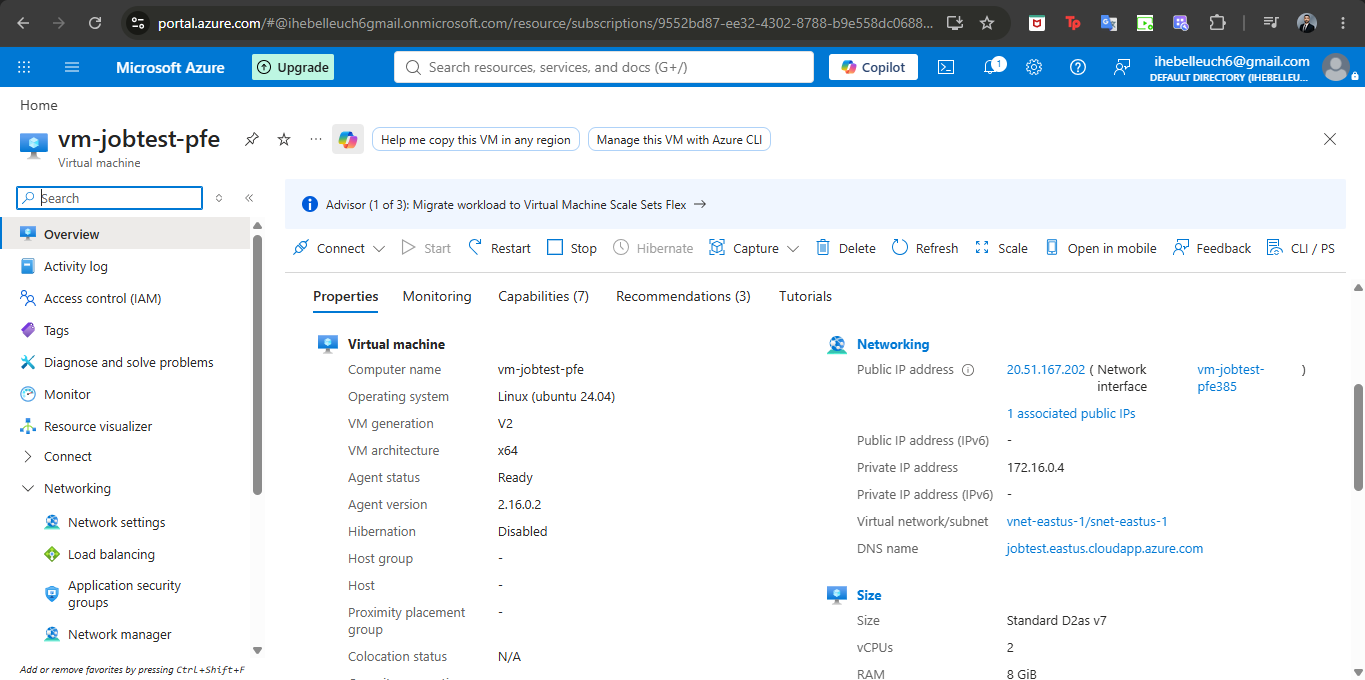
\includegraphics[width=.82\textwidth,trim=0 0 0 105bp,clip]{img/azure/azure_vm1.png}
  \caption{Propriétés observées de la machine virtuelle}
  \label{fig:chap6-azure-vm-properties}
\end{figure}

Son état d'exécution apparaît sur la figure~\ref{fig:chap6-azure-vm-state}.

\begin{figure}[H]
  \centering
  \begin{tikzpicture}[baseline=(image.base)]
    \node[anchor=south west,inner sep=0] (image) at (0,0) {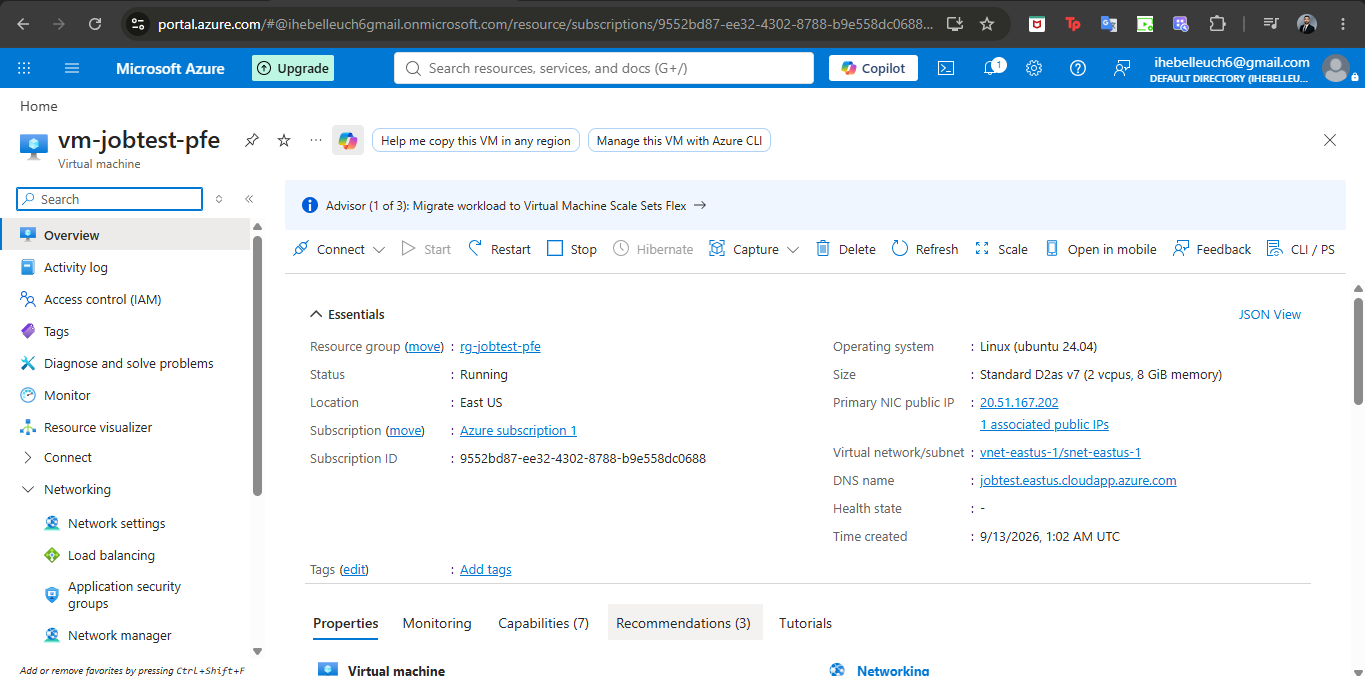
\includegraphics[width=.82\textwidth,trim=0 0 0 105bp,clip]{img/azure/azure_vm2.png}};
    \fill[white] (4.36,2.02) rectangle (8.88,2.63);
    \node[font=\tiny] at (6.62,2.32) {masqué};
  \end{tikzpicture}
  \caption{État de la machine virtuelle, recadré}
  \label{fig:chap6-azure-vm-state}
\end{figure}

La figure~\ref{fig:chap6-azure-ip} montre enfin la ressource d'adresse IP publique rattachée à la machine.

\begin{figure}[H]
  \centering
  \begin{tikzpicture}[baseline=(image.base)]
    \node[anchor=south west,inner sep=0] (image) at (0,0) {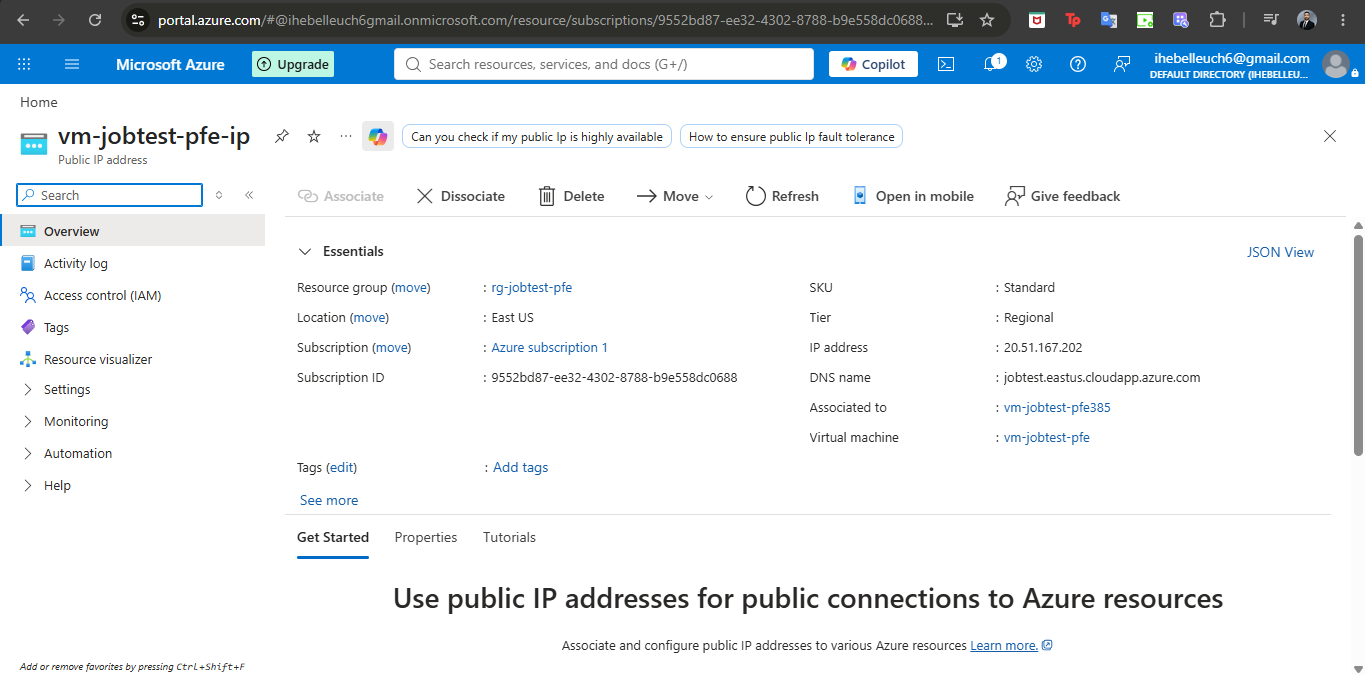
\includegraphics[width=.82\textwidth,trim=0 0 0 105bp,clip]{img/azure/azure ip.png}};
    \fill[white] (4.36,2.53) rectangle (8.88,3.14);
    \node[font=\tiny] at (6.62,2.84) {masqué};
  \end{tikzpicture}
  \caption{Ressource d'adresse IP publique, recadrée}
  \label{fig:chap6-azure-ip}
\end{figure}

Le format D2as\_v7 a été retenu comme compromis pour une démonstration de PFE et pour l'exécution locale de \texttt{qwen2.5:1.5b}. Il n'est pas dimensionné pour une charge réelle soutenue : la latence de la couche 2 sur CPU illustre cette contrainte. La création précise de la règle NSG et son niveau d'attachement n'ont pas été archivés ; seul son effet, l'accès HTTP externe, est confirmé.

\section{Architecture de déploiement}

La figure \ref{fig:chap6-deployment} matérialise les trois frontières utiles à l'exploitation : Azure filtre l'entrée publique, la VM héberge le proxy et le réseau Docker porte les communications de service à service. Les volumes \texttt{postgres\_data}, \texttt{ollama\_data} et \texttt{embedding\_cache} séparent les données persistantes des conteneurs recréables. Le navigateur ne communique ni avec PostgreSQL, ni avec Ollama, ni directement avec FastAPI ou Next.js : il atteint Nginx, qui distribue ensuite les routes internes.

\section{Exploitation et maîtrise des coûts}

Le contexte de démonstration mentionne un crédit Azure Free Trial de 200 USD, sans calcul mensuel figé : le coût affiché dépend de la région, du temps d'allocation et des ressources associées. L'arrêt automatique est activé mais ne doit pas être assimilé sans vérification à une désallocation. Microsoft indique que la fonctionnalité d'auto-arrêt est configurable selon un horaire et un fuseau horaire \cite{azure_auto_shutdown}. Après une démonstration, il faut contrôler l'état réel de la VM et privilégier \emph{Stop (deallocate)} pour libérer le calcul. Le disque et, selon sa configuration, l'adresse IP peuvent continuer à générer des coûts ; la persistance de ces ressources explique qu'une désallocation ne soit pas une suppression.

\section{Procédures d'exploitation}

Les commandes suivantes correspondent aux opérations prévues par la procédure de déploiement. Elles ne révèlent pas le contenu de l'environnement ni les secrets.

\begin{verbatim}
cd /opt/jobtest
docker compose ps
docker compose logs --tail=200 nginx api web ollama db
docker compose restart
docker compose up -d --build
docker compose down
docker compose exec -T db sh -c 'pg_dump -U "$POSTGRES_USER" "$POSTGRES_DB"' | gzip > jobtest-backup.sql.gz
\end{verbatim}

La dernière commande est la forme documentée de sauvegarde PostgreSQL. La commande \texttt{docker compose down} arrête les conteneurs tout en conservant les volumes nommés ; l'option \texttt{-v} n'est donc pas utilisée, car elle supprimerait les données persistantes et les caches.

\section{Bilan du déploiement}

Le tableau~\ref{tab:chap6-deployment-summary} met en regard chaque résultat observé et la limite qui l'accompagne.

\begin{table}[H]
\centering
\small
\caption{Synthèse des résultats observés et des limites}
\label{tab:chap6-deployment-summary}
\begin{tabularx}{\textwidth}{|p{.18\textwidth}|X|X|}
\hline
\textbf{Élément} & \textbf{Résultat observé} & \textbf{Limite}\\
\hline
Interface Next.js & Accessible derrière Nginx. & HTTP uniquement.\\
\hline
API FastAPI & Santé et routes publiques de démonstration disponibles. & Ressources CPU/RAM limitées.\\
\hline
PostgreSQL & Persistance d'un résultat et d'une analyse validée. & Sauvegarde à automatiser.\\
\hline
Couche 1 & Évaluation et explication fonctionnelles. & Validation réelle avec recruteurs encore nécessaire.\\
\hline
Couche 2 & Analyse \texttt{ok} disponible. & Latence CPU élevée ; contenu consultatif.\\
\hline
PDF & Export valide sur un exemple de deux pages. & Test ponctuel, taille variable.\\
\hline
Réseau & Ports applicatifs internes non publiés. & SSH à restreindre ; UFW inactif observé.\\
\hline
Disponibilité & Démonstration réussie avec cinq services sains. & VM unique, sans haute disponibilité.\\
\hline
\end{tabularx}
\end{table}

\section*{Conclusion}

Les preuves réunies confirment le fonctionnement d'une chaîne complète de démonstration : l'évaluation, la persistance, l'analyse qualitative et l'export PDF sont servis par une pile conteneurisée, avec Nginx comme point d'entrée et des services métier non publiés directement. Le déploiement Azure est donc opérationnel dans son périmètre de PFE. Il ne constitue toutefois ni une certification de sécurité ni une infrastructure de production : HTTPS, le durcissement de SSH, les sauvegardes, la supervision et la tolérance aux pannes restent à mettre en œuvre. Ces résultats permettent de replacer, dans la conclusion générale, les apports du prototype et les conditions de son évolution.
